\documentclass{book}
\usepackage[a4paper,top=2.5cm,bottom=2.5cm,left=2.5cm,right=2.5cm]{geometry}
\usepackage{makeidx}
\usepackage{natbib}
\usepackage{graphicx}
\usepackage{multicol}
\usepackage{float}
\usepackage{listings}
\usepackage{color}
\usepackage{ifthen}
\usepackage[table]{xcolor}
\usepackage{textcomp}
\usepackage{alltt}
\usepackage{ifpdf}
\ifpdf
\usepackage[pdftex,
            pagebackref=true,
            colorlinks=true,
            linkcolor=blue,
            unicode
           ]{hyperref}
\else
\usepackage[ps2pdf,
            pagebackref=true,
            colorlinks=true,
            linkcolor=blue,
            unicode
           ]{hyperref}
\usepackage{pspicture}
\fi
\usepackage[utf8]{inputenc}
\usepackage{polski}
\usepackage[T1]{fontenc}

\usepackage{mathptmx}
\usepackage[scaled=.90]{helvet}
\usepackage{courier}
\usepackage{sectsty}
\usepackage{amssymb}
\usepackage[titles]{tocloft}
\usepackage{doxygen}
\lstset{language=C++,inputencoding=utf8,basicstyle=\footnotesize,breaklines=true,breakatwhitespace=true,tabsize=4,numbers=left }
\makeindex
\setcounter{tocdepth}{3}
\renewcommand{\footrulewidth}{0.4pt}
\renewcommand{\familydefault}{\sfdefault}
\hfuzz=15pt
\setlength{\emergencystretch}{15pt}
\hbadness=750
\tolerance=750
\begin{document}
\hypersetup{pageanchor=false,citecolor=blue}
\begin{titlepage}
\vspace*{7cm}
\begin{center}
{\Large Swift\-:\-:Engine }\\
\vspace*{1cm}
{\large Wygenerowano przez Doxygen 1.8.3.1}\\
\vspace*{0.5cm}
{\small Pn, 29 kwi 2013 00:06:12}\\
\end{center}
\end{titlepage}
\clearemptydoublepage
\pagenumbering{roman}
\tableofcontents
\clearemptydoublepage
\pagenumbering{arabic}
\hypersetup{pageanchor=true,citecolor=blue}
\chapter{Indeks hierarchiczny}
\section{Hierarchia klas}
Ta lista dziedziczenia posortowana jest z grubsza, choć nie całkowicie, alfabetycznie\-:\begin{DoxyCompactList}
\item \contentsline{section}{Swift\-:\-:Camera}{\pageref{class_swift_1_1_camera}}{}
\item \contentsline{section}{Swift\-:\-:Glfw\-Window}{\pageref{class_swift_1_1_glfw_window}}{}
\item \contentsline{section}{Swift\-:\-:Group}{\pageref{class_swift_1_1_group}}{}
\item \contentsline{section}{Swift\-:\-:Material}{\pageref{class_swift_1_1_material}}{}
\item \contentsline{section}{Swift\-:\-:Material\-Manager\-Class}{\pageref{class_swift_1_1_material_manager_class}}{}
\item \contentsline{section}{Swift\-:\-:Object}{\pageref{class_swift_1_1_object}}{}
\begin{DoxyCompactList}
\item \contentsline{section}{Swift\-:\-:Cube}{\pageref{class_swift_1_1_cube}}{}
\item \contentsline{section}{Swift\-:\-:Mesh}{\pageref{class_swift_1_1_mesh}}{}
\item \contentsline{section}{Swift\-:\-:Plane}{\pageref{class_swift_1_1_plane}}{}
\item \contentsline{section}{Swift\-:\-:Sphere}{\pageref{class_swift_1_1_sphere}}{}
\end{DoxyCompactList}
\item \contentsline{section}{Swift\-:\-:Object\-Manager\-Class}{\pageref{class_swift_1_1_object_manager_class}}{}
\item \contentsline{section}{Swift\-:\-:Renderer}{\pageref{class_swift_1_1_renderer}}{}
\item \contentsline{section}{Singleton$<$ T $>$}{\pageref{class_singleton}}{}
\item \contentsline{section}{Supervisor}{\pageref{class_supervisor}}{}
\item \contentsline{section}{Swift\-:\-:Supervisor\-Class}{\pageref{class_swift_1_1_supervisor_class}}{}
\end{DoxyCompactList}

\chapter{Indeks klas}
\section{Lista klas}
Tutaj znajdują się klasy, struktury, unie i interfejsy wraz z ich krótkimi opisami\-:\begin{DoxyCompactList}
\item\contentsline{section}{\hyperlink{class_swift_1_1_camera}{Swift\-::\-Camera} }{\pageref{class_swift_1_1_camera}}{}
\item\contentsline{section}{\hyperlink{class_swift_1_1_cube}{Swift\-::\-Cube} }{\pageref{class_swift_1_1_cube}}{}
\item\contentsline{section}{\hyperlink{class_swift_1_1_glfw_window}{Swift\-::\-Glfw\-Window} }{\pageref{class_swift_1_1_glfw_window}}{}
\item\contentsline{section}{\hyperlink{class_swift_1_1_group}{Swift\-::\-Group} }{\pageref{class_swift_1_1_group}}{}
\item\contentsline{section}{\hyperlink{class_swift_1_1_material}{Swift\-::\-Material} }{\pageref{class_swift_1_1_material}}{}
\item\contentsline{section}{\hyperlink{class_swift_1_1_material_manager_class}{Swift\-::\-Material\-Manager\-Class} }{\pageref{class_swift_1_1_material_manager_class}}{}
\item\contentsline{section}{\hyperlink{class_swift_1_1_mesh}{Swift\-::\-Mesh} }{\pageref{class_swift_1_1_mesh}}{}
\item\contentsline{section}{\hyperlink{class_swift_1_1_object}{Swift\-::\-Object} }{\pageref{class_swift_1_1_object}}{}
\item\contentsline{section}{\hyperlink{class_swift_1_1_object_manager_class}{Swift\-::\-Object\-Manager\-Class} }{\pageref{class_swift_1_1_object_manager_class}}{}
\item\contentsline{section}{\hyperlink{class_swift_1_1_plane}{Swift\-::\-Plane} }{\pageref{class_swift_1_1_plane}}{}
\item\contentsline{section}{\hyperlink{class_swift_1_1_renderer}{Swift\-::\-Renderer} }{\pageref{class_swift_1_1_renderer}}{}
\item\contentsline{section}{\hyperlink{class_singleton}{Singleton$<$ T $>$} }{\pageref{class_singleton}}{}
\item\contentsline{section}{\hyperlink{class_swift_1_1_sphere}{Swift\-::\-Sphere} }{\pageref{class_swift_1_1_sphere}}{}
\item\contentsline{section}{\hyperlink{class_supervisor}{Supervisor} \\*Klasa-\/singleton, która pozwala na dostęp do funkcji ogólnych (sprawdzenie wersji itp.) + daje dostęp do innych singletonów (Object\-Manager, Material\-Manager itp.) }{\pageref{class_supervisor}}{}
\item\contentsline{section}{\hyperlink{class_swift_1_1_supervisor_class}{Swift\-::\-Supervisor\-Class} }{\pageref{class_swift_1_1_supervisor_class}}{}
\end{DoxyCompactList}

\chapter{Indeks plików}
\section{Lista plików}
Tutaj znajduje się lista wszystkich udokumentowanych plików z ich krótkimi opisami\-:\begin{DoxyCompactList}
\item\contentsline{section}{include/\hyperlink{_camera_8h}{Camera.\-h} }{\pageref{_camera_8h}}{}
\item\contentsline{section}{include/{\bfseries Cube.\-h} }{\pageref{_cube_8h}}{}
\item\contentsline{section}{include/{\bfseries Glfw\-Window.\-h} }{\pageref{_glfw_window_8h}}{}
\item\contentsline{section}{include/{\bfseries Group.\-h} }{\pageref{_group_8h}}{}
\item\contentsline{section}{include/{\bfseries Handle.\-h} }{\pageref{_handle_8h}}{}
\item\contentsline{section}{include/{\bfseries Handle\-Manager.\-h} }{\pageref{_handle_manager_8h}}{}
\item\contentsline{section}{include/{\bfseries Material.\-h} }{\pageref{_material_8h}}{}
\item\contentsline{section}{include/{\bfseries Material\-Manager.\-h} }{\pageref{_material_manager_8h}}{}
\item\contentsline{section}{include/{\bfseries Mesh.\-h} }{\pageref{_mesh_8h}}{}
\item\contentsline{section}{include/{\bfseries Object.\-h} }{\pageref{_object_8h}}{}
\item\contentsline{section}{include/{\bfseries Object\-Manager.\-h} }{\pageref{_object_manager_8h}}{}
\item\contentsline{section}{include/{\bfseries Plane.\-h} }{\pageref{_plane_8h}}{}
\item\contentsline{section}{include/{\bfseries Renderer.\-h} }{\pageref{_renderer_8h}}{}
\item\contentsline{section}{include/{\bfseries Singleton.\-h} }{\pageref{_singleton_8h}}{}
\item\contentsline{section}{include/{\bfseries Sphere.\-h} }{\pageref{_sphere_8h}}{}
\item\contentsline{section}{include/\hyperlink{_supervisor_8h}{Supervisor.\-h} \\*Zawiera definicję klasy nadzorcy która daje dostęp do najważniejszych nagłówków i najważniejszych funkcji, których nie dało się wrzucić nigdzie indziej }{\pageref{_supervisor_8h}}{}
\end{DoxyCompactList}

\chapter{Dokumentacja klas}
\hypertarget{class_swift_1_1_camera}{\section{Dokumentacja klasy Swift\-:\-:Camera}
\label{class_swift_1_1_camera}\index{Swift\-::\-Camera@{Swift\-::\-Camera}}
}
\subsection*{Metody publiczne}
\begin{DoxyCompactItemize}
\item 
void \hyperlink{class_swift_1_1_camera_a1deb0323f01dc0f4f4c8339a7f08ccec}{refresh} ()
\item 
void \hyperlink{class_swift_1_1_camera_afbf0a7b7684200d7535fb21af76f4d0f}{set\-Fo\-V} (const float \&\-\_\-fov)
\item 
void \hyperlink{class_swift_1_1_camera_aec504f41e362e79dfee84fb9dd21afff}{set\-Aspect} (const float \&\-\_\-aspect)
\item 
void \hyperlink{class_swift_1_1_camera_a67e483588f775f2cc1a8d95edd7098d1}{set\-Near\-Clip} (const float \&\-\_\-near\-Clip)
\item 
void \hyperlink{class_swift_1_1_camera_af55fb7e3056753e91e6663c19c535907}{set\-Far\-Clip} (const float \&\-\_\-far\-Clip)
\item 
void \hyperlink{class_swift_1_1_camera_adef87453165bf6a77e75473572ffd123}{set\-View\-Params} (glm\-::vec3 \-\_\-pos, glm\-::vec3 \-\_\-target, glm\-::vec3 \-\_\-up)
\item 
\hypertarget{class_swift_1_1_camera_a5ab2155a81e1e71cfe0d0a2eec613327}{void {\bfseries set\-Projection\-Params} (const float \&\-\_\-fov, const float \&\-\_\-aspect, const float \&\-\_\-near\-Clip, const float \&\-\_\-far\-Clip)}\label{class_swift_1_1_camera_a5ab2155a81e1e71cfe0d0a2eec613327}

\item 
\hypertarget{class_swift_1_1_camera_a63ebeba2a56eb6e1e71294b902d08aef}{void {\bfseries set\-View\-Matrix} (const glm\-::mat4 \&\-\_\-\-View)}\label{class_swift_1_1_camera_a63ebeba2a56eb6e1e71294b902d08aef}

\item 
\hypertarget{class_swift_1_1_camera_a29e1b6b95af09c1fa6d4525ddad561ff}{void {\bfseries set\-Projection\-Matrix} (const glm\-::mat4 \&\-\_\-\-Projection)}\label{class_swift_1_1_camera_a29e1b6b95af09c1fa6d4525ddad561ff}

\item 
\hypertarget{class_swift_1_1_camera_a14de6f59dab7997977103ab497668e9a}{glm\-::mat4 {\bfseries get\-V\-P} ()}\label{class_swift_1_1_camera_a14de6f59dab7997977103ab497668e9a}

\item 
glm\-::mat4 \hyperlink{class_swift_1_1_camera_a6fb94d155749b0169ef2ed79302ad414}{get\-View} ()
\item 
glm\-::mat4 \hyperlink{class_swift_1_1_camera_a56f048c36a97568a52f1ac56a76f28b9}{get\-Projection} ()
\item 
float \hyperlink{class_swift_1_1_camera_a44dd87522fbf1373d27a75a5118ded1f}{get\-Fo\-V} ()
\item 
float \hyperlink{class_swift_1_1_camera_ab1d5d6f54d38bd4a1ed634b8ddbaaeb8}{get\-Aspect} ()
\item 
\hypertarget{class_swift_1_1_camera_a2516e737315e7baa9be4cc2f3d5d89f2}{float {\bfseries get\-Near\-Clip} ()}\label{class_swift_1_1_camera_a2516e737315e7baa9be4cc2f3d5d89f2}

\item 
\hypertarget{class_swift_1_1_camera_a671fcaedeb7403344be02cba61e07828}{float {\bfseries get\-Far\-Clip} ()}\label{class_swift_1_1_camera_a671fcaedeb7403344be02cba61e07828}

\item 
\hypertarget{class_swift_1_1_camera_af7ece7b2345142287ebb8f44c9bfc4e8}{glm\-::vec3 {\bfseries get\-Position} ()}\label{class_swift_1_1_camera_af7ece7b2345142287ebb8f44c9bfc4e8}

\item 
\hypertarget{class_swift_1_1_camera_a81a20875b877e888eb4303cdd921e648}{glm\-::vec3 {\bfseries get\-Target} ()}\label{class_swift_1_1_camera_a81a20875b877e888eb4303cdd921e648}

\item 
\hypertarget{class_swift_1_1_camera_a444610e566bcf79edae4431142ac1840}{glm\-::vec3 {\bfseries get\-Up\-Vector} ()}\label{class_swift_1_1_camera_a444610e566bcf79edae4431142ac1840}

\item 
\hypertarget{class_swift_1_1_camera_a8a1b0e633e0325d30b44f473b8c88f87}{void {\bfseries move} (const glm\-::vec3 \&\-\_\-pos, const glm\-::vec3 \&offset, const glm\-::vec3 \&\-\_\-up, float \-\_\-fov=45.\-0f)}\label{class_swift_1_1_camera_a8a1b0e633e0325d30b44f473b8c88f87}

\item 
\hyperlink{class_swift_1_1_camera_a2670e9e2fd99c38790b92e568bbadfda}{Camera} (glm\-::vec3 \-\_\-pos, glm\-::vec3 \-\_\-target, glm\-::vec3 \-\_\-up, const float \&\-\_\-fov, const float \&\-\_\-aspect, const float \&\-\_\-near\-Clip, const float \&\-\_\-far\-Clip)
\end{DoxyCompactItemize}


\subsection{Dokumentacja konstruktora i destruktora}
\hypertarget{class_swift_1_1_camera_a2670e9e2fd99c38790b92e568bbadfda}{\index{Swift\-::\-Camera@{Swift\-::\-Camera}!Camera@{Camera}}
\index{Camera@{Camera}!Swift::Camera@{Swift\-::\-Camera}}
\subsubsection[{Camera}]{\setlength{\rightskip}{0pt plus 5cm}Swift\-::\-Camera\-::\-Camera (
\begin{DoxyParamCaption}
\item[{glm\-::vec3}]{\-\_\-pos, }
\item[{glm\-::vec3}]{\-\_\-target, }
\item[{glm\-::vec3}]{\-\_\-up, }
\item[{const float \&}]{\-\_\-fov, }
\item[{const float \&}]{\-\_\-aspect, }
\item[{const float \&}]{\-\_\-near\-Clip, }
\item[{const float \&}]{\-\_\-far\-Clip}
\end{DoxyParamCaption}
)}}\label{class_swift_1_1_camera_a2670e9e2fd99c38790b92e568bbadfda}
Basic constructor -\/ sets View and Perspective to identity matrices; use O\-N\-L\-Y when you intend to change the paramters later and refresh matrices manually by using \hyperlink{class_swift_1_1_camera_a1deb0323f01dc0f4f4c8339a7f08ccec}{Camera\-::refresh()} 

\subsection{Dokumentacja funkcji składowych}
\hypertarget{class_swift_1_1_camera_ab1d5d6f54d38bd4a1ed634b8ddbaaeb8}{\index{Swift\-::\-Camera@{Swift\-::\-Camera}!get\-Aspect@{get\-Aspect}}
\index{get\-Aspect@{get\-Aspect}!Swift::Camera@{Swift\-::\-Camera}}
\subsubsection[{get\-Aspect}]{\setlength{\rightskip}{0pt plus 5cm}float Swift\-::\-Camera\-::get\-Aspect (
\begin{DoxyParamCaption}
{}
\end{DoxyParamCaption}
)}}\label{class_swift_1_1_camera_ab1d5d6f54d38bd4a1ed634b8ddbaaeb8}
Get Field of View value \hypertarget{class_swift_1_1_camera_a44dd87522fbf1373d27a75a5118ded1f}{\index{Swift\-::\-Camera@{Swift\-::\-Camera}!get\-Fo\-V@{get\-Fo\-V}}
\index{get\-Fo\-V@{get\-Fo\-V}!Swift::Camera@{Swift\-::\-Camera}}
\subsubsection[{get\-Fo\-V}]{\setlength{\rightskip}{0pt plus 5cm}float Swift\-::\-Camera\-::get\-Fo\-V (
\begin{DoxyParamCaption}
{}
\end{DoxyParamCaption}
)}}\label{class_swift_1_1_camera_a44dd87522fbf1373d27a75a5118ded1f}
Get Projection Matrix \hypertarget{class_swift_1_1_camera_a56f048c36a97568a52f1ac56a76f28b9}{\index{Swift\-::\-Camera@{Swift\-::\-Camera}!get\-Projection@{get\-Projection}}
\index{get\-Projection@{get\-Projection}!Swift::Camera@{Swift\-::\-Camera}}
\subsubsection[{get\-Projection}]{\setlength{\rightskip}{0pt plus 5cm}glm\-::mat4 Swift\-::\-Camera\-::get\-Projection (
\begin{DoxyParamCaption}
{}
\end{DoxyParamCaption}
)}}\label{class_swift_1_1_camera_a56f048c36a97568a52f1ac56a76f28b9}
Get View matrix \hypertarget{class_swift_1_1_camera_a6fb94d155749b0169ef2ed79302ad414}{\index{Swift\-::\-Camera@{Swift\-::\-Camera}!get\-View@{get\-View}}
\index{get\-View@{get\-View}!Swift::Camera@{Swift\-::\-Camera}}
\subsubsection[{get\-View}]{\setlength{\rightskip}{0pt plus 5cm}glm\-::mat4 Swift\-::\-Camera\-::get\-View (
\begin{DoxyParamCaption}
{}
\end{DoxyParamCaption}
)}}\label{class_swift_1_1_camera_a6fb94d155749b0169ef2ed79302ad414}
Get View$\ast$\-Projection matrix \hypertarget{class_swift_1_1_camera_a1deb0323f01dc0f4f4c8339a7f08ccec}{\index{Swift\-::\-Camera@{Swift\-::\-Camera}!refresh@{refresh}}
\index{refresh@{refresh}!Swift::Camera@{Swift\-::\-Camera}}
\subsubsection[{refresh}]{\setlength{\rightskip}{0pt plus 5cm}void Swift\-::\-Camera\-::refresh (
\begin{DoxyParamCaption}
{}
\end{DoxyParamCaption}
)}}\label{class_swift_1_1_camera_a1deb0323f01dc0f4f4c8339a7f08ccec}
Projection matrix -\/ deforms the object to create perspective \hypertarget{class_swift_1_1_camera_aec504f41e362e79dfee84fb9dd21afff}{\index{Swift\-::\-Camera@{Swift\-::\-Camera}!set\-Aspect@{set\-Aspect}}
\index{set\-Aspect@{set\-Aspect}!Swift::Camera@{Swift\-::\-Camera}}
\subsubsection[{set\-Aspect}]{\setlength{\rightskip}{0pt plus 5cm}void Swift\-::\-Camera\-::set\-Aspect (
\begin{DoxyParamCaption}
\item[{const float \&}]{\-\_\-aspect}
\end{DoxyParamCaption}
)}}\label{class_swift_1_1_camera_aec504f41e362e79dfee84fb9dd21afff}
Set F\-O\-V value \hypertarget{class_swift_1_1_camera_af55fb7e3056753e91e6663c19c535907}{\index{Swift\-::\-Camera@{Swift\-::\-Camera}!set\-Far\-Clip@{set\-Far\-Clip}}
\index{set\-Far\-Clip@{set\-Far\-Clip}!Swift::Camera@{Swift\-::\-Camera}}
\subsubsection[{set\-Far\-Clip}]{\setlength{\rightskip}{0pt plus 5cm}void Swift\-::\-Camera\-::set\-Far\-Clip (
\begin{DoxyParamCaption}
\item[{const float \&}]{\-\_\-far\-Clip}
\end{DoxyParamCaption}
)}}\label{class_swift_1_1_camera_af55fb7e3056753e91e6663c19c535907}
Set Near Clipping value \hypertarget{class_swift_1_1_camera_afbf0a7b7684200d7535fb21af76f4d0f}{\index{Swift\-::\-Camera@{Swift\-::\-Camera}!set\-Fo\-V@{set\-Fo\-V}}
\index{set\-Fo\-V@{set\-Fo\-V}!Swift::Camera@{Swift\-::\-Camera}}
\subsubsection[{set\-Fo\-V}]{\setlength{\rightskip}{0pt plus 5cm}void Swift\-::\-Camera\-::set\-Fo\-V (
\begin{DoxyParamCaption}
\item[{const float \&}]{\-\_\-fov}
\end{DoxyParamCaption}
)}}\label{class_swift_1_1_camera_afbf0a7b7684200d7535fb21af76f4d0f}
Refresh matrices after parameter change \hypertarget{class_swift_1_1_camera_a67e483588f775f2cc1a8d95edd7098d1}{\index{Swift\-::\-Camera@{Swift\-::\-Camera}!set\-Near\-Clip@{set\-Near\-Clip}}
\index{set\-Near\-Clip@{set\-Near\-Clip}!Swift::Camera@{Swift\-::\-Camera}}
\subsubsection[{set\-Near\-Clip}]{\setlength{\rightskip}{0pt plus 5cm}void Swift\-::\-Camera\-::set\-Near\-Clip (
\begin{DoxyParamCaption}
\item[{const float \&}]{\-\_\-near\-Clip}
\end{DoxyParamCaption}
)}}\label{class_swift_1_1_camera_a67e483588f775f2cc1a8d95edd7098d1}
Set the screen aspect ratio \hypertarget{class_swift_1_1_camera_adef87453165bf6a77e75473572ffd123}{\index{Swift\-::\-Camera@{Swift\-::\-Camera}!set\-View\-Params@{set\-View\-Params}}
\index{set\-View\-Params@{set\-View\-Params}!Swift::Camera@{Swift\-::\-Camera}}
\subsubsection[{set\-View\-Params}]{\setlength{\rightskip}{0pt plus 5cm}void Swift\-::\-Camera\-::set\-View\-Params (
\begin{DoxyParamCaption}
\item[{glm\-::vec3}]{\-\_\-pos, }
\item[{glm\-::vec3}]{\-\_\-target, }
\item[{glm\-::vec3}]{\-\_\-up}
\end{DoxyParamCaption}
)}}\label{class_swift_1_1_camera_adef87453165bf6a77e75473572ffd123}
Set Far Clipping value 

Dokumentacja dla tej klasy została wygenerowana z plików\-:\begin{DoxyCompactItemize}
\item 
include/\hyperlink{_camera_8h}{Camera.\-h}\item 
src/Camera.\-cpp\end{DoxyCompactItemize}

\hypertarget{class_swift_1_1_cube}{\section{Dokumentacja klasy Swift\-:\-:Cube}
\label{class_swift_1_1_cube}\index{Swift\-::\-Cube@{Swift\-::\-Cube}}
}
Diagram dziedziczenia dla Swift\-:\-:Cube\begin{figure}[H]
\begin{center}
\leavevmode
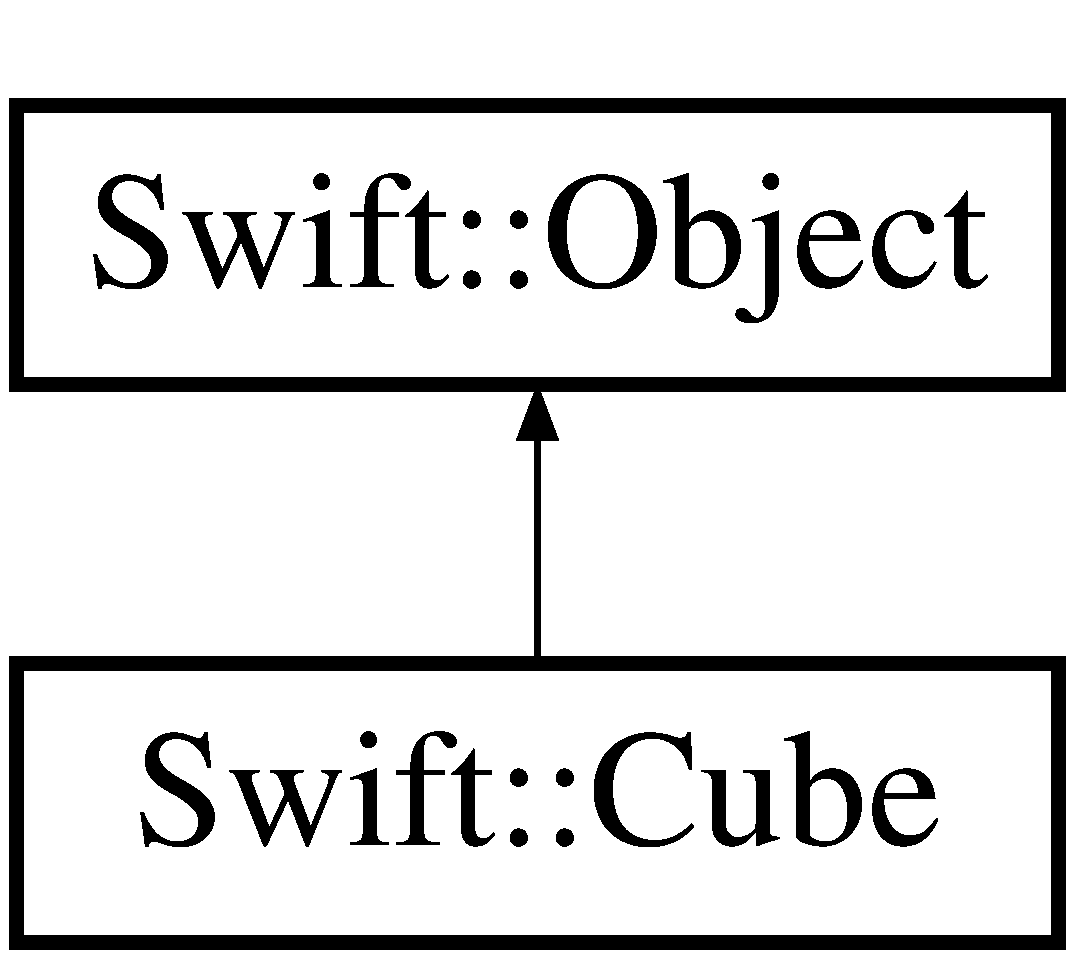
\includegraphics[height=2.000000cm]{class_swift_1_1_cube}
\end{center}
\end{figure}
\subsection*{Metody publiczne}
\begin{DoxyCompactItemize}
\item 
\hypertarget{class_swift_1_1_cube_ae293fe3bde8e707a707d20e5ec586bbb}{int {\bfseries get\-Seg\-Count} ()}\label{class_swift_1_1_cube_ae293fe3bde8e707a707d20e5ec586bbb}

\item 
\hypertarget{class_swift_1_1_cube_a0837a0bfcc83b68ba5c6af78744f1170}{void {\bfseries set\-Seg\-Count} (int count)}\label{class_swift_1_1_cube_a0837a0bfcc83b68ba5c6af78744f1170}

\item 
\hypertarget{class_swift_1_1_cube_a44067639fb2828ae4f6445d9f261e2af}{void {\bfseries set\-Side} (int \-\_\-a)}\label{class_swift_1_1_cube_a44067639fb2828ae4f6445d9f261e2af}

\item 
\hypertarget{class_swift_1_1_cube_a5b1c3243362c4ec37d654d6fd9d65b87}{{\bfseries Cube} (int \-\_\-a, const glm\-::vec3 \&\-\_\-pos, int \-\_\-segs=1)}\label{class_swift_1_1_cube_a5b1c3243362c4ec37d654d6fd9d65b87}

\end{DoxyCompactItemize}
\subsection*{Metody chronione}
\begin{DoxyCompactItemize}
\item 
\hypertarget{class_swift_1_1_cube_a491f12450d538c885d9a0a5e08afac94}{void {\bfseries calculate\-Vertices} ()}\label{class_swift_1_1_cube_a491f12450d538c885d9a0a5e08afac94}

\end{DoxyCompactItemize}
\subsection*{Atrybuty chronione}
\begin{DoxyCompactItemize}
\item 
\hypertarget{class_swift_1_1_cube_ada2febc703f56b7cb623e114656a9fc0}{int {\bfseries segs}}\label{class_swift_1_1_cube_ada2febc703f56b7cb623e114656a9fc0}

\item 
\hypertarget{class_swift_1_1_cube_a7e8e1e2d724967ce411274db7052134f}{int {\bfseries a}}\label{class_swift_1_1_cube_a7e8e1e2d724967ce411274db7052134f}

\end{DoxyCompactItemize}


Dokumentacja dla tej klasy została wygenerowana z plików\-:\begin{DoxyCompactItemize}
\item 
include/Cube.\-h\item 
src/Cube.\-cpp\end{DoxyCompactItemize}

\hypertarget{class_swift_1_1_glfw_window}{\section{Dokumentacja klasy Swift\-:\-:Glfw\-Window}
\label{class_swift_1_1_glfw_window}\index{Swift\-::\-Glfw\-Window@{Swift\-::\-Glfw\-Window}}
}
\subsection*{Metody publiczne}
\begin{DoxyCompactItemize}
\item 
\hypertarget{class_swift_1_1_glfw_window_a293e3df4b7f81dcd5a2e293d0c0a0e6e}{void {\bfseries swap\-Buffers} ()}\label{class_swift_1_1_glfw_window_a293e3df4b7f81dcd5a2e293d0c0a0e6e}

\item 
\hypertarget{class_swift_1_1_glfw_window_a3e2d2767424b07351f6bd31b936c5fb0}{bool {\bfseries is\-Open} ()}\label{class_swift_1_1_glfw_window_a3e2d2767424b07351f6bd31b936c5fb0}

\item 
\hypertarget{class_swift_1_1_glfw_window_a96d3d541d3f7988e2575adbfa2dca51f}{int {\bfseries get\-Width} ()}\label{class_swift_1_1_glfw_window_a96d3d541d3f7988e2575adbfa2dca51f}

\item 
\hypertarget{class_swift_1_1_glfw_window_ac563261a4c5d7df87c36638e9d6edae1}{int {\bfseries get\-Height} ()}\label{class_swift_1_1_glfw_window_ac563261a4c5d7df87c36638e9d6edae1}

\item 
\hypertarget{class_swift_1_1_glfw_window_a2b0892ae66e4daef8489de02539e679d}{std\-::string {\bfseries get\-Title} ()}\label{class_swift_1_1_glfw_window_a2b0892ae66e4daef8489de02539e679d}

\item 
\hypertarget{class_swift_1_1_glfw_window_af165765a36d8dc9c471c081052644f1c}{int {\bfseries get\-F\-S\-A\-Asamples} ()}\label{class_swift_1_1_glfw_window_af165765a36d8dc9c471c081052644f1c}

\item 
\hypertarget{class_swift_1_1_glfw_window_ab6ef902af7b79a40e01df82c165a499f}{int {\bfseries get\-Mode} ()}\label{class_swift_1_1_glfw_window_ab6ef902af7b79a40e01df82c165a499f}

\item 
\hypertarget{class_swift_1_1_glfw_window_af8c667c8845cf9d20614a19d6b6f2a92}{void {\bfseries set\-Mode} (int m)}\label{class_swift_1_1_glfw_window_af8c667c8845cf9d20614a19d6b6f2a92}

\item 
\hypertarget{class_swift_1_1_glfw_window_a2804a109453b35535e6406f3a1fbed8a}{void {\bfseries set\-F\-S\-A\-Asamples} (int count)}\label{class_swift_1_1_glfw_window_a2804a109453b35535e6406f3a1fbed8a}

\item 
\hypertarget{class_swift_1_1_glfw_window_aaedfd8e1dcdfcff6aa83af2d29603a64}{void {\bfseries set\-Title} (std\-::string t)}\label{class_swift_1_1_glfw_window_aaedfd8e1dcdfcff6aa83af2d29603a64}

\item 
\hypertarget{class_swift_1_1_glfw_window_a7190075f5f829fc42bc4ed3f23feccad}{void {\bfseries set\-Width} (int w)}\label{class_swift_1_1_glfw_window_a7190075f5f829fc42bc4ed3f23feccad}

\item 
\hypertarget{class_swift_1_1_glfw_window_a1b9659f332299689e3b6097ec36bf911}{void {\bfseries set\-Height} (int h)}\label{class_swift_1_1_glfw_window_a1b9659f332299689e3b6097ec36bf911}

\item 
\hypertarget{class_swift_1_1_glfw_window_a809d12ff5711c10bd12ccb5ca067eef7}{{\bfseries Glfw\-Window} (int w, int h, int m, std\-::string t=\char`\"{}Swift\-::\-Engine example application\char`\"{})}\label{class_swift_1_1_glfw_window_a809d12ff5711c10bd12ccb5ca067eef7}

\end{DoxyCompactItemize}


Dokumentacja dla tej klasy została wygenerowana z plików\-:\begin{DoxyCompactItemize}
\item 
include/Glfw\-Window.\-h\item 
src/Glfw\-Window.\-cpp\end{DoxyCompactItemize}

\hypertarget{class_swift_1_1_group}{\section{Dokumentacja klasy Swift\-:\-:Group}
\label{class_swift_1_1_group}\index{Swift\-::\-Group@{Swift\-::\-Group}}
}
\subsection*{Metody publiczne}
\begin{DoxyCompactItemize}
\item 
\hypertarget{class_swift_1_1_group_afce53738ef8d6f6e5d175efb9732aae9}{void {\bfseries add} (\hyperlink{class_swift_1_1_object}{Object} $\ast$obj)}\label{class_swift_1_1_group_afce53738ef8d6f6e5d175efb9732aae9}

\item 
\hypertarget{class_swift_1_1_group_a69675968ef7a0aff30b9bde563c4c049}{void {\bfseries remove} (std\-::string \-\_\-name)}\label{class_swift_1_1_group_a69675968ef7a0aff30b9bde563c4c049}

\item 
\hypertarget{class_swift_1_1_group_ae2e53956668341cde2e1f54143f9934b}{void {\bfseries remove\-At} (unsigned int index)}\label{class_swift_1_1_group_ae2e53956668341cde2e1f54143f9934b}

\item 
\hypertarget{class_swift_1_1_group_a8003af9fcc0277b6c7b6d55573f6aa6c}{std\-::vector$<$ \hyperlink{class_swift_1_1_object}{Object} $\ast$ $>$ $\ast$ {\bfseries get\-Objects} ()}\label{class_swift_1_1_group_a8003af9fcc0277b6c7b6d55573f6aa6c}

\item 
\hypertarget{class_swift_1_1_group_ae4fc910a6f9382bed12e2d76bb51c3fe}{void {\bfseries set\-Name} (std\-::string \-\_\-name)}\label{class_swift_1_1_group_ae4fc910a6f9382bed12e2d76bb51c3fe}

\item 
\hypertarget{class_swift_1_1_group_a6228adf834b941c85cdb780229150af8}{std\-::string {\bfseries get\-Name} ()}\label{class_swift_1_1_group_a6228adf834b941c85cdb780229150af8}

\item 
\hypertarget{class_swift_1_1_group_ae454e92e2b6bd7bbcd868a0a2a02eff7}{\hyperlink{class_swift_1_1_object}{Object} $\ast$ {\bfseries get\-Object} (std\-::string \-\_\-name)}\label{class_swift_1_1_group_ae454e92e2b6bd7bbcd868a0a2a02eff7}

\item 
\hypertarget{class_swift_1_1_group_a7bce81ad79cd9c9198c74b6a18437c07}{\hyperlink{class_swift_1_1_object}{Object} $\ast$ {\bfseries get\-Object\-At} (unsigned int index)}\label{class_swift_1_1_group_a7bce81ad79cd9c9198c74b6a18437c07}

\item 
\hypertarget{class_swift_1_1_group_a56c2ddd378894060b15038159ec0e08d}{{\bfseries Group} (\hyperlink{class_swift_1_1_object}{Object} $\ast$obj)}\label{class_swift_1_1_group_a56c2ddd378894060b15038159ec0e08d}

\end{DoxyCompactItemize}


Dokumentacja dla tej klasy została wygenerowana z plików\-:\begin{DoxyCompactItemize}
\item 
include/Group.\-h\item 
src/Group.\-cpp\end{DoxyCompactItemize}

\hypertarget{class_swift_1_1_material}{\section{Dokumentacja klasy Swift\-:\-:Material}
\label{class_swift_1_1_material}\index{Swift\-::\-Material@{Swift\-::\-Material}}
}
\subsection*{Metody publiczne}
\begin{DoxyCompactItemize}
\item 
\hypertarget{class_swift_1_1_material_af9684f28734d244487c8442f6f32ad70}{void {\bfseries set\-Shader} (std\-::string name)}\label{class_swift_1_1_material_af9684f28734d244487c8442f6f32ad70}

\item 
\hypertarget{class_swift_1_1_material_aba83259cef5253597dd401913024ccac}{G\-Luint {\bfseries get\-Shader\-I\-D} ()}\label{class_swift_1_1_material_aba83259cef5253597dd401913024ccac}

\item 
\hypertarget{class_swift_1_1_material_a89b8a632f2da253bddcb3dec996e1ee8}{{\bfseries Material} (std\-::string shader\-Name)}\label{class_swift_1_1_material_a89b8a632f2da253bddcb3dec996e1ee8}

\end{DoxyCompactItemize}


Dokumentacja dla tej klasy została wygenerowana z plików\-:\begin{DoxyCompactItemize}
\item 
include/Material.\-h\item 
src/Material.\-cpp\end{DoxyCompactItemize}

\hypertarget{class_swift_1_1_material_manager_class}{\section{Dokumentacja klasy Swift\-:\-:Material\-Manager\-Class}
\label{class_swift_1_1_material_manager_class}\index{Swift\-::\-Material\-Manager\-Class@{Swift\-::\-Material\-Manager\-Class}}
}
\subsection*{Metody publiczne}
\begin{DoxyCompactItemize}
\item 
\hypertarget{class_swift_1_1_material_manager_class_aeb13a6288bf4966107bc7a7e31c80518}{void {\bfseries load\-Shader} (std\-::string shader\-\_\-name, std\-::string vertex\-\_\-shader\-\_\-name, std\-::string pixel\-\_\-shader\-\_\-name)}\label{class_swift_1_1_material_manager_class_aeb13a6288bf4966107bc7a7e31c80518}

\item 
\hypertarget{class_swift_1_1_material_manager_class_aeaee837ceb85f2453a231671549b3a93}{unsigned int {\bfseries get\-Shader} (std\-::string name)}\label{class_swift_1_1_material_manager_class_aeaee837ceb85f2453a231671549b3a93}

\end{DoxyCompactItemize}


Dokumentacja dla tej klasy została wygenerowana z plików\-:\begin{DoxyCompactItemize}
\item 
include/Material\-Manager.\-h\item 
src/Material\-Manager.\-cpp\end{DoxyCompactItemize}

\hypertarget{class_swift_1_1_mesh}{\section{Dokumentacja klasy Swift\-:\-:Mesh}
\label{class_swift_1_1_mesh}\index{Swift\-::\-Mesh@{Swift\-::\-Mesh}}
}
Diagram dziedziczenia dla Swift\-:\-:Mesh\begin{figure}[H]
\begin{center}
\leavevmode
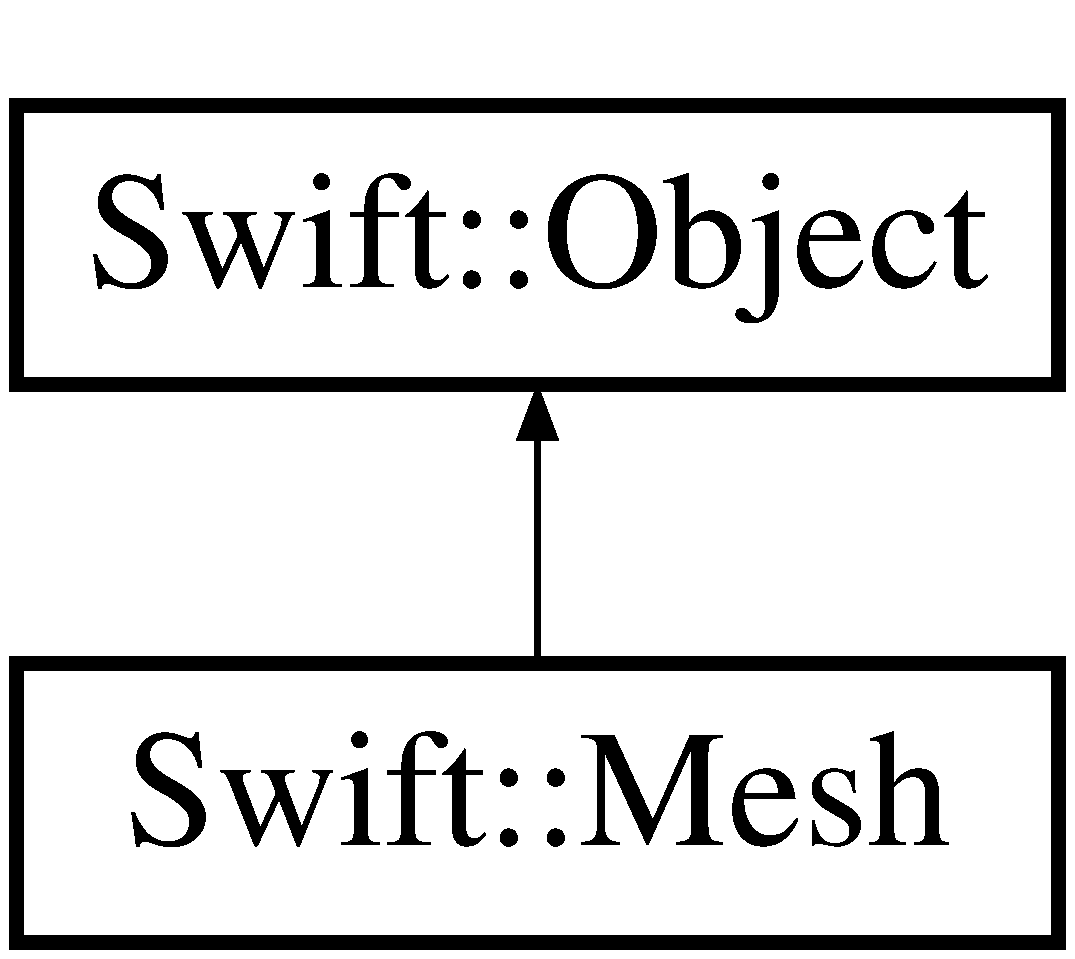
\includegraphics[height=2.000000cm]{class_swift_1_1_mesh}
\end{center}
\end{figure}
\subsection*{Metody publiczne}
\begin{DoxyCompactItemize}
\item 
\hypertarget{class_swift_1_1_mesh_ac6572f81c093dce1a16a452eaf2121dd}{void {\bfseries load\-Obj} (const char $\ast$filename)}\label{class_swift_1_1_mesh_ac6572f81c093dce1a16a452eaf2121dd}

\item 
\hypertarget{class_swift_1_1_mesh_a9fdf742b0dda4c81ba421d131feb4007}{void {\bfseries load3\-D\-S} (const char $\ast$filename)}\label{class_swift_1_1_mesh_a9fdf742b0dda4c81ba421d131feb4007}

\item 
\hypertarget{class_swift_1_1_mesh_ac0294d75b61631d73dbef1925de2473c}{void {\bfseries load\-Blend} (const char $\ast$filename)}\label{class_swift_1_1_mesh_ac0294d75b61631d73dbef1925de2473c}

\item 
\hypertarget{class_swift_1_1_mesh_adaf53c5aa90edbba32b125339192fec5}{{\bfseries Mesh} (const glm\-::vec3 \&pos=glm\-::vec3(0, 0, 0))}\label{class_swift_1_1_mesh_adaf53c5aa90edbba32b125339192fec5}

\item 
\hypertarget{class_swift_1_1_mesh_ac613e4ca2c1bbb16b885b4a5bff8840c}{{\bfseries Mesh} (const char $\ast$filename, const glm\-::vec3 \&pos=glm\-::vec3(0, 0, 0))}\label{class_swift_1_1_mesh_ac613e4ca2c1bbb16b885b4a5bff8840c}

\end{DoxyCompactItemize}
\subsection*{Dodatkowe Dziedziczone Składowe}


Dokumentacja dla tej klasy została wygenerowana z plików\-:\begin{DoxyCompactItemize}
\item 
include/Mesh.\-h\item 
src/Mesh.\-cpp\end{DoxyCompactItemize}

\hypertarget{class_swift_1_1_object}{\section{Dokumentacja klasy Swift\-:\-:Object}
\label{class_swift_1_1_object}\index{Swift\-::\-Object@{Swift\-::\-Object}}
}
Diagram dziedziczenia dla Swift\-:\-:Object\begin{figure}[H]
\begin{center}
\leavevmode
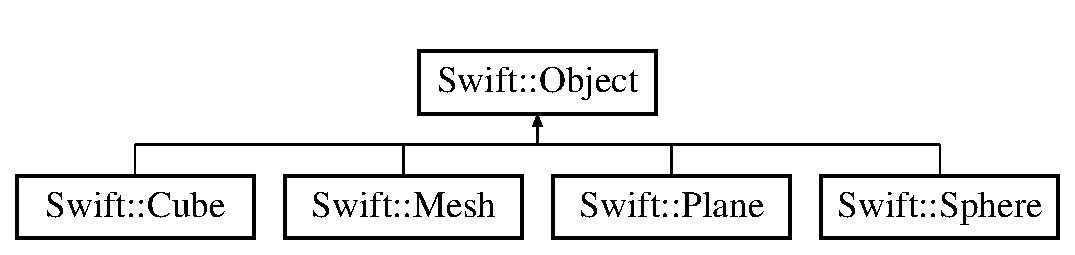
\includegraphics[height=2.000000cm]{class_swift_1_1_object}
\end{center}
\end{figure}
\subsection*{Metody publiczne}
\begin{DoxyCompactItemize}
\item 
\hypertarget{class_swift_1_1_object_a1ccd0029126c7da038cb15e815c6a14c}{G\-Lfloat $\ast$ {\bfseries get\-Vertices} ()}\label{class_swift_1_1_object_a1ccd0029126c7da038cb15e815c6a14c}

\item 
\hypertarget{class_swift_1_1_object_ad1b89bd12733960c02cad14f8a276093}{\hyperlink{class_swift_1_1_material}{Material} $\ast$ {\bfseries get\-Material} ()}\label{class_swift_1_1_object_ad1b89bd12733960c02cad14f8a276093}

\item 
\hypertarget{class_swift_1_1_object_ac261dd2051c68f8024f3b901805d3a04}{glm\-::mat4 {\bfseries get\-Model\-Matrix} ()}\label{class_swift_1_1_object_ac261dd2051c68f8024f3b901805d3a04}

\item 
\hypertarget{class_swift_1_1_object_a148b13cce13e533935d8e0800b1b04f0}{glm\-::vec3 {\bfseries get\-Position} ()}\label{class_swift_1_1_object_a148b13cce13e533935d8e0800b1b04f0}

\item 
\hypertarget{class_swift_1_1_object_a4ec2b118a5fe6de5bed9cbd4b52edf7d}{glm\-::vec3 {\bfseries get\-Origin} ()}\label{class_swift_1_1_object_a4ec2b118a5fe6de5bed9cbd4b52edf7d}

\item 
\hypertarget{class_swift_1_1_object_a2b4b91289fd15c3b7454d46e443365d6}{bool {\bfseries is\-Visible} ()}\label{class_swift_1_1_object_a2b4b91289fd15c3b7454d46e443365d6}

\item 
\hypertarget{class_swift_1_1_object_a022cce5050ec8be6b3f3f6463d870e9d}{void {\bfseries hide} ()}\label{class_swift_1_1_object_a022cce5050ec8be6b3f3f6463d870e9d}

\item 
\hypertarget{class_swift_1_1_object_ab64474800ccf9a7d85a6d009da9cd309}{void {\bfseries show} ()}\label{class_swift_1_1_object_ab64474800ccf9a7d85a6d009da9cd309}

\item 
\hypertarget{class_swift_1_1_object_a1789c833984c0fabaefa53b77381f5f7}{unsigned int {\bfseries get\-Vertex\-Count} ()}\label{class_swift_1_1_object_a1789c833984c0fabaefa53b77381f5f7}

\item 
\hypertarget{class_swift_1_1_object_a0ad97a59eba18ce2ab2c2f78ad7a14bb}{void {\bfseries rotate} (const glm\-::vec3 \&axis, float angle)}\label{class_swift_1_1_object_a0ad97a59eba18ce2ab2c2f78ad7a14bb}

\item 
\hypertarget{class_swift_1_1_object_a1b85f8ad0b60b47c97df22de669802a0}{void {\bfseries move} (const glm\-::vec3 \&new\-Pos)}\label{class_swift_1_1_object_a1b85f8ad0b60b47c97df22de669802a0}

\item 
\hypertarget{class_swift_1_1_object_ad9ac8b7d237f712224e99f17e0c05550}{void {\bfseries scale} (const glm\-::vec3 \&factor)}\label{class_swift_1_1_object_ad9ac8b7d237f712224e99f17e0c05550}

\item 
\hypertarget{class_swift_1_1_object_a1cac75564cd937ba90bc4401adfe27b5}{G\-Luint {\bfseries get\-V\-B\-O} ()}\label{class_swift_1_1_object_a1cac75564cd937ba90bc4401adfe27b5}

\item 
\hypertarget{class_swift_1_1_object_ac72cd5fa7364e1722d13bc68ac66743d}{G\-Luint {\bfseries get\-V\-A\-O} ()}\label{class_swift_1_1_object_ac72cd5fa7364e1722d13bc68ac66743d}

\item 
\hypertarget{class_swift_1_1_object_a8504beacff2b73bfb3532e40e8b685c0}{G\-Luint {\bfseries get\-Normal\-Buffer} ()}\label{class_swift_1_1_object_a8504beacff2b73bfb3532e40e8b685c0}

\item 
\hypertarget{class_swift_1_1_object_a5e2dc8186cb2f201f7fc71174a99e282}{G\-Luint {\bfseries get\-U\-Vbuffer} ()}\label{class_swift_1_1_object_a5e2dc8186cb2f201f7fc71174a99e282}

\item 
\hypertarget{class_swift_1_1_object_a50721e35e58987d0952785de8ca05297}{void {\bfseries set\-Name} (std\-::string \-\_\-name)}\label{class_swift_1_1_object_a50721e35e58987d0952785de8ca05297}

\item 
\hypertarget{class_swift_1_1_object_ad3449afb41a15af0523d2e73a165a25b}{void {\bfseries set\-Material} (\hyperlink{class_swift_1_1_material}{Material} $\ast$\-\_\-mtl)}\label{class_swift_1_1_object_ad3449afb41a15af0523d2e73a165a25b}

\item 
\hypertarget{class_swift_1_1_object_a0bd304548c71364a63702c458e28bcd3}{std\-::string {\bfseries get\-Name} ()}\label{class_swift_1_1_object_a0bd304548c71364a63702c458e28bcd3}

\end{DoxyCompactItemize}
\subsection*{Metody chronione}
\begin{DoxyCompactItemize}
\item 
\hypertarget{class_swift_1_1_object_a5fdcff5fc9eedd88e9d6b6374f7cc865}{void {\bfseries destroy} ()}\label{class_swift_1_1_object_a5fdcff5fc9eedd88e9d6b6374f7cc865}

\item 
\hypertarget{class_swift_1_1_object_a1732ea6a4c30701e80e2abdc00035cef}{void {\bfseries setup} ()}\label{class_swift_1_1_object_a1732ea6a4c30701e80e2abdc00035cef}

\item 
\hypertarget{class_swift_1_1_object_ae10d931f1c4bf41b6b2376b4a7d53312}{void {\bfseries reload} ()}\label{class_swift_1_1_object_ae10d931f1c4bf41b6b2376b4a7d53312}

\end{DoxyCompactItemize}
\subsection*{Atrybuty chronione}
\begin{DoxyCompactItemize}
\item 
\hypertarget{class_swift_1_1_object_a8f8676d34bb644d23f18b940d11c1086}{glm\-::mat4 {\bfseries Model}}\label{class_swift_1_1_object_a8f8676d34bb644d23f18b940d11c1086}

\item 
\hypertarget{class_swift_1_1_object_a35139111d8e8e784f311d8cca95d68c4}{glm\-::vec3 {\bfseries origin}}\label{class_swift_1_1_object_a35139111d8e8e784f311d8cca95d68c4}

\item 
\hypertarget{class_swift_1_1_object_a6c801de7abc9b6bb694d958fe0876543}{G\-Luint {\bfseries V\-B\-O}}\label{class_swift_1_1_object_a6c801de7abc9b6bb694d958fe0876543}

\item 
\hypertarget{class_swift_1_1_object_a3fae7f32130c46c2b76aefae3c6aa1e7}{G\-Luint {\bfseries V\-A\-O}}\label{class_swift_1_1_object_a3fae7f32130c46c2b76aefae3c6aa1e7}

\item 
\hypertarget{class_swift_1_1_object_a5029da6cf367b9e34c62daa45a4a56c2}{G\-Luint {\bfseries normalbuffer}}\label{class_swift_1_1_object_a5029da6cf367b9e34c62daa45a4a56c2}

\item 
\hypertarget{class_swift_1_1_object_a2373549381ac70c984cedbf40b06d85c}{G\-Luint {\bfseries uvbuffer}}\label{class_swift_1_1_object_a2373549381ac70c984cedbf40b06d85c}

\item 
\hypertarget{class_swift_1_1_object_a8a1161446d212565e63daa50f472da0f}{std\-::vector$<$ glm\-::vec3 $>$ {\bfseries vertices}}\label{class_swift_1_1_object_a8a1161446d212565e63daa50f472da0f}

\item 
\hypertarget{class_swift_1_1_object_a8bc1f0d82ee32b85a3164eb8d3282cb5}{std\-::vector$<$ glm\-::vec2 $>$ {\bfseries uvs}}\label{class_swift_1_1_object_a8bc1f0d82ee32b85a3164eb8d3282cb5}

\item 
\hypertarget{class_swift_1_1_object_a6448734d9a42316c0f7c57b859856eff}{std\-::vector$<$ glm\-::vec3 $>$ {\bfseries normals}}\label{class_swift_1_1_object_a6448734d9a42316c0f7c57b859856eff}

\item 
\hypertarget{class_swift_1_1_object_abb53e36006fdbdd3650781663e79a46c}{std\-::string {\bfseries name}}\label{class_swift_1_1_object_abb53e36006fdbdd3650781663e79a46c}

\item 
\hypertarget{class_swift_1_1_object_ae9ad394a8ecaf399d781fa677a091f9b}{\hyperlink{class_swift_1_1_material}{Material} $\ast$ {\bfseries mtl}}\label{class_swift_1_1_object_ae9ad394a8ecaf399d781fa677a091f9b}

\item 
\hypertarget{class_swift_1_1_object_a378504148dfbad4d67a25d682d83702b}{bool {\bfseries visible}}\label{class_swift_1_1_object_a378504148dfbad4d67a25d682d83702b}

\end{DoxyCompactItemize}


Dokumentacja dla tej klasy została wygenerowana z plików\-:\begin{DoxyCompactItemize}
\item 
include/Object.\-h\item 
src/Object.\-cpp\end{DoxyCompactItemize}

\hypertarget{class_swift_1_1_object_manager_class}{\section{Dokumentacja klasy Swift\-:\-:Object\-Manager\-Class}
\label{class_swift_1_1_object_manager_class}\index{Swift\-::\-Object\-Manager\-Class@{Swift\-::\-Object\-Manager\-Class}}
}
\subsection*{Metody publiczne}
\begin{DoxyCompactItemize}
\item 
\hypertarget{class_swift_1_1_object_manager_class_a613685184bf09809d44a698850d4aa61}{void {\bfseries add} (\hyperlink{class_swift_1_1_group}{Group} $\ast$\-\_\-group)}\label{class_swift_1_1_object_manager_class_a613685184bf09809d44a698850d4aa61}

\item 
\hypertarget{class_swift_1_1_object_manager_class_a10ef742475be3476a93866d7fe32427d}{void {\bfseries remove} (std\-::string name)}\label{class_swift_1_1_object_manager_class_a10ef742475be3476a93866d7fe32427d}

\item 
\hypertarget{class_swift_1_1_object_manager_class_ad418717cc92d60410da844555c4c0268}{void {\bfseries remove\-At} (unsigned int index)}\label{class_swift_1_1_object_manager_class_ad418717cc92d60410da844555c4c0268}

\item 
\hypertarget{class_swift_1_1_object_manager_class_ac906673364d5d11003d2f2a4b4e35ae0}{std\-::vector$<$ \hyperlink{class_swift_1_1_group}{Group} $\ast$ $>$ $\ast$ {\bfseries get\-Groups} ()}\label{class_swift_1_1_object_manager_class_ac906673364d5d11003d2f2a4b4e35ae0}

\end{DoxyCompactItemize}


Dokumentacja dla tej klasy została wygenerowana z plików\-:\begin{DoxyCompactItemize}
\item 
include/Object\-Manager.\-h\item 
src/Object\-Manager.\-cpp\end{DoxyCompactItemize}

\hypertarget{class_swift_1_1_plane}{\section{Dokumentacja klasy Swift\-:\-:Plane}
\label{class_swift_1_1_plane}\index{Swift\-::\-Plane@{Swift\-::\-Plane}}
}
Diagram dziedziczenia dla Swift\-:\-:Plane\begin{figure}[H]
\begin{center}
\leavevmode
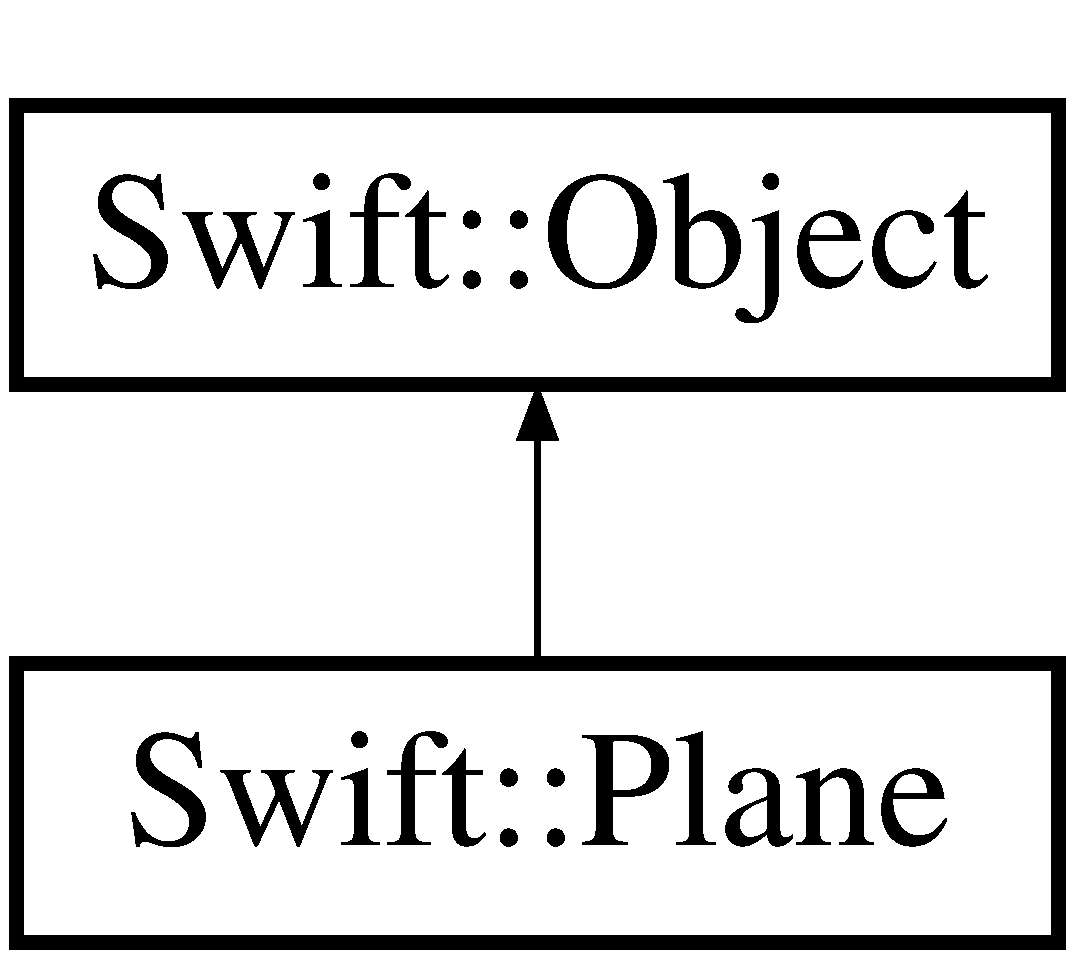
\includegraphics[height=2.000000cm]{class_swift_1_1_plane}
\end{center}
\end{figure}
\subsection*{Metody publiczne}
\begin{DoxyCompactItemize}
\item 
\hypertarget{class_swift_1_1_plane_a5f654ef9113bea684b53328caf120576}{int {\bfseries get\-Height\-Seg\-Count} ()}\label{class_swift_1_1_plane_a5f654ef9113bea684b53328caf120576}

\item 
\hypertarget{class_swift_1_1_plane_a4a2d32e4549496070fb86872c4b6d034}{int {\bfseries get\-Width\-Seg\-Count} ()}\label{class_swift_1_1_plane_a4a2d32e4549496070fb86872c4b6d034}

\item 
\hypertarget{class_swift_1_1_plane_a0b258151162b09301bea59bfaf595be7}{double {\bfseries get\-Width} ()}\label{class_swift_1_1_plane_a0b258151162b09301bea59bfaf595be7}

\item 
\hypertarget{class_swift_1_1_plane_a7fec527ad2fed8741b1fcc52df1431f4}{double {\bfseries get\-Height} ()}\label{class_swift_1_1_plane_a7fec527ad2fed8741b1fcc52df1431f4}

\item 
\hypertarget{class_swift_1_1_plane_acf9e20528202f5ddef83d392f9a49f6b}{void {\bfseries set\-Height\-Seg\-Count} (int count)}\label{class_swift_1_1_plane_acf9e20528202f5ddef83d392f9a49f6b}

\item 
\hypertarget{class_swift_1_1_plane_a06235c599ac0cf3b56d131906af9ecad}{void {\bfseries set\-Width\-Seg\-Count} (int count)}\label{class_swift_1_1_plane_a06235c599ac0cf3b56d131906af9ecad}

\item 
\hypertarget{class_swift_1_1_plane_a2adbe3c8324ccf6b248a5adb77f50b2f}{{\bfseries Plane} (double \-\_\-width, double \-\_\-height, const glm\-::vec3 \&pos=glm\-::vec3(0, 0, 0), int height\-Segments=1, int width\-Segments=1)}\label{class_swift_1_1_plane_a2adbe3c8324ccf6b248a5adb77f50b2f}

\end{DoxyCompactItemize}
\subsection*{Metody chronione}
\begin{DoxyCompactItemize}
\item 
\hypertarget{class_swift_1_1_plane_a2a91b7615a5905cbf23c77b4802eac95}{void {\bfseries calculate\-Vertices} ()}\label{class_swift_1_1_plane_a2a91b7615a5905cbf23c77b4802eac95}

\end{DoxyCompactItemize}
\subsection*{Atrybuty chronione}
\begin{DoxyCompactItemize}
\item 
\hypertarget{class_swift_1_1_plane_aeb428fb89663547df455e8f4f5a63086}{int {\bfseries height\-Segs}}\label{class_swift_1_1_plane_aeb428fb89663547df455e8f4f5a63086}

\item 
\hypertarget{class_swift_1_1_plane_a5620fcdf357be2c71506a3688adb2f58}{int {\bfseries width\-Segs}}\label{class_swift_1_1_plane_a5620fcdf357be2c71506a3688adb2f58}

\item 
\hypertarget{class_swift_1_1_plane_a9098b81cd7e15b866a4ae9f77fdcfd79}{double {\bfseries width}}\label{class_swift_1_1_plane_a9098b81cd7e15b866a4ae9f77fdcfd79}

\item 
\hypertarget{class_swift_1_1_plane_aa5ddc56c4285b3aa3da7340aef2757d3}{double {\bfseries height}}\label{class_swift_1_1_plane_aa5ddc56c4285b3aa3da7340aef2757d3}

\end{DoxyCompactItemize}


Dokumentacja dla tej klasy została wygenerowana z plików\-:\begin{DoxyCompactItemize}
\item 
include/Plane.\-h\item 
src/Plane.\-cpp\end{DoxyCompactItemize}

\hypertarget{class_swift_1_1_renderer}{\section{Dokumentacja klasy Swift\-:\-:Renderer}
\label{class_swift_1_1_renderer}\index{Swift\-::\-Renderer@{Swift\-::\-Renderer}}
}
\subsection*{Metody publiczne}
\begin{DoxyCompactItemize}
\item 
\hypertarget{class_swift_1_1_renderer_abdde0957ffcda6dff1f36473b3d4729f}{void {\bfseries render} ()}\label{class_swift_1_1_renderer_abdde0957ffcda6dff1f36473b3d4729f}

\item 
\hypertarget{class_swift_1_1_renderer_af44e3cdc0e9f3cefb5a576ab873806bc}{void {\bfseries set\-Camera} (\hyperlink{class_swift_1_1_camera}{Camera} $\ast$c)}\label{class_swift_1_1_renderer_af44e3cdc0e9f3cefb5a576ab873806bc}

\item 
\hypertarget{class_swift_1_1_renderer_a87e97312cc9816407510a19ea6449a6c}{void {\bfseries set\-Render\-Mode} (unsigned int mode)}\label{class_swift_1_1_renderer_a87e97312cc9816407510a19ea6449a6c}

\item 
\hypertarget{class_swift_1_1_renderer_a16000bca04395354b6450a9a920e4884}{int {\bfseries get\-Render\-Mode} ()}\label{class_swift_1_1_renderer_a16000bca04395354b6450a9a920e4884}

\item 
\hypertarget{class_swift_1_1_renderer_ae3c63586d9ef1546deb8eedac24710ec}{void {\bfseries clear\-Color} (double r, double g, double b, double a)}\label{class_swift_1_1_renderer_ae3c63586d9ef1546deb8eedac24710ec}

\end{DoxyCompactItemize}


Dokumentacja dla tej klasy została wygenerowana z plików\-:\begin{DoxyCompactItemize}
\item 
include/Renderer.\-h\item 
src/Renderer.\-cpp\end{DoxyCompactItemize}

\hypertarget{class_singleton}{\section{Dokumentacja szablonu klasy Singleton$<$ T $>$}
\label{class_singleton}\index{Singleton$<$ T $>$@{Singleton$<$ T $>$}}
}
\subsection*{Statyczne metody publiczne}
\begin{DoxyCompactItemize}
\item 
\hypertarget{class_singleton_aac3d56c39edc2b596260b787f9aef758}{static T $\ast$ {\bfseries get\-Singleton} ()}\label{class_singleton_aac3d56c39edc2b596260b787f9aef758}

\end{DoxyCompactItemize}


Dokumentacja dla tej klasy została wygenerowana z pliku\-:\begin{DoxyCompactItemize}
\item 
include/Singleton.\-h\end{DoxyCompactItemize}

\hypertarget{class_swift_1_1_sphere}{\section{Dokumentacja klasy Swift\-:\-:Sphere}
\label{class_swift_1_1_sphere}\index{Swift\-::\-Sphere@{Swift\-::\-Sphere}}
}
Diagram dziedziczenia dla Swift\-:\-:Sphere\begin{figure}[H]
\begin{center}
\leavevmode
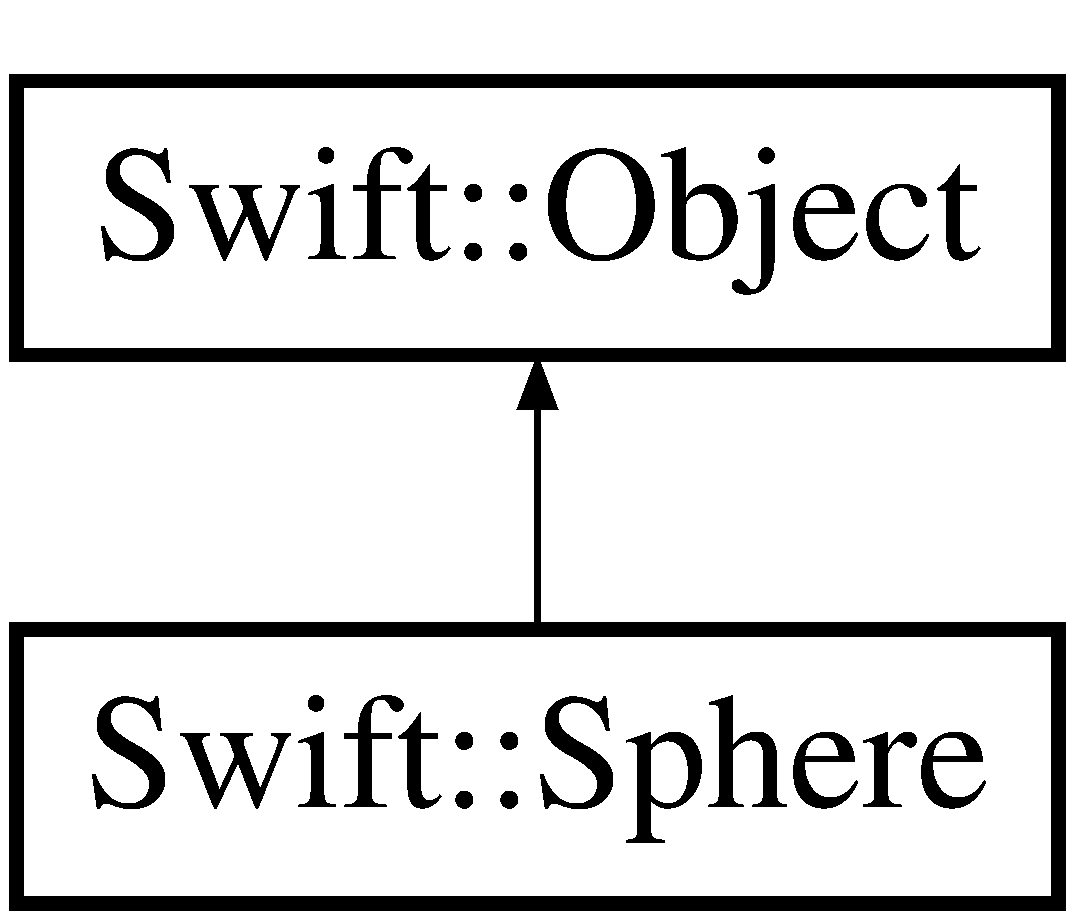
\includegraphics[height=2.000000cm]{class_swift_1_1_sphere}
\end{center}
\end{figure}
\subsection*{Metody publiczne}
\begin{DoxyCompactItemize}
\item 
\hypertarget{class_swift_1_1_sphere_a98b0f80678d54067f1b074289a220a08}{int {\bfseries get\-Segment\-Count} ()}\label{class_swift_1_1_sphere_a98b0f80678d54067f1b074289a220a08}

\item 
\hypertarget{class_swift_1_1_sphere_a252444234c0405da50fbb6a68574beba}{double {\bfseries get\-Radius} ()}\label{class_swift_1_1_sphere_a252444234c0405da50fbb6a68574beba}

\item 
\hypertarget{class_swift_1_1_sphere_af733f1fccaf3cd10ac6f36bbefb70d36}{int {\bfseries get\-Ring\-Count} ()}\label{class_swift_1_1_sphere_af733f1fccaf3cd10ac6f36bbefb70d36}

\item 
\hypertarget{class_swift_1_1_sphere_a8a611c6724d168cbec468e5eff28001f}{void {\bfseries set\-Segment\-Count} (int \-\_\-segments)}\label{class_swift_1_1_sphere_a8a611c6724d168cbec468e5eff28001f}

\item 
\hypertarget{class_swift_1_1_sphere_acfc2322a46181ddfa54a39023c032f6b}{void {\bfseries set\-Ring\-Count} (int \-\_\-rings)}\label{class_swift_1_1_sphere_acfc2322a46181ddfa54a39023c032f6b}

\item 
\hypertarget{class_swift_1_1_sphere_a1dc49ee4d701b304b0dc81862e72cc9c}{void {\bfseries set\-Radius} (double \-\_\-radius)}\label{class_swift_1_1_sphere_a1dc49ee4d701b304b0dc81862e72cc9c}

\item 
\hypertarget{class_swift_1_1_sphere_a553289d5fcf34b8ce82d205efecf190d}{{\bfseries Sphere} (double \-\_\-radius, int \-\_\-segments, int \-\_\-rings, glm\-::vec3 center)}\label{class_swift_1_1_sphere_a553289d5fcf34b8ce82d205efecf190d}

\end{DoxyCompactItemize}
\subsection*{Dodatkowe Dziedziczone Składowe}


Dokumentacja dla tej klasy została wygenerowana z plików\-:\begin{DoxyCompactItemize}
\item 
include/Sphere.\-h\item 
src/Sphere.\-cpp\end{DoxyCompactItemize}

\hypertarget{class_supervisor}{\section{Dokumentacja klasy Supervisor}
\label{class_supervisor}\index{Supervisor@{Supervisor}}
}


Klasa-\/singleton, która pozwala na dostęp do funkcji ogólnych (sprawdzenie wersji itp.) + daje dostęp do innych singletonów (Object\-Manager, Material\-Manager itp.)  




{\ttfamily \#include $<$Supervisor.\-h$>$}



\subsection{Opis szczegółowy}
Klasa-\/singleton, która pozwala na dostęp do funkcji ogólnych (sprawdzenie wersji itp.) + daje dostęp do innych singletonów (Object\-Manager, Material\-Manager itp.) 

Dokumentacja dla tej klasy została wygenerowana z pliku\-:\begin{DoxyCompactItemize}
\item 
include/\hyperlink{_supervisor_8h}{Supervisor.\-h}\end{DoxyCompactItemize}

\hypertarget{class_swift_1_1_supervisor_class}{\section{Dokumentacja klasy Swift\-:\-:Supervisor\-Class}
\label{class_swift_1_1_supervisor_class}\index{Swift\-::\-Supervisor\-Class@{Swift\-::\-Supervisor\-Class}}
}
\subsection*{Metody publiczne}
\begin{DoxyCompactItemize}
\item 
std\-::string \hyperlink{class_swift_1_1_supervisor_class_a61de186286647e800f29daaa0ee1c4f2}{get\-Renderer} ()
\item 
std\-::string \hyperlink{class_swift_1_1_supervisor_class_ad34493aab889bc6b02de096fb5a91438}{get\-Open\-G\-Lversion} ()
\item 
std\-::string \hyperlink{class_swift_1_1_supervisor_class_afef1724b416b8fc506a6683dc427fb23}{get\-Vendor} ()
\item 
std\-::string \hyperlink{class_swift_1_1_supervisor_class_a7c04ed59b515b69cc84926fc3b697a8e}{get\-Shader\-Language\-Version} ()
\item 
\hyperlink{class_swift_1_1_supervisor_class_a7859add3cb374988faa7d290d0cec628}{Supervisor\-Class} ()
\item 
\hyperlink{class_swift_1_1_supervisor_class_ae280bf97af5a687cd29feee26288d33b}{$\sim$\-Supervisor\-Class} ()
\end{DoxyCompactItemize}


\subsection{Dokumentacja konstruktora i destruktora}
\hypertarget{class_swift_1_1_supervisor_class_a7859add3cb374988faa7d290d0cec628}{\index{Swift\-::\-Supervisor\-Class@{Swift\-::\-Supervisor\-Class}!Supervisor\-Class@{Supervisor\-Class}}
\index{Supervisor\-Class@{Supervisor\-Class}!Swift::SupervisorClass@{Swift\-::\-Supervisor\-Class}}
\subsubsection[{Supervisor\-Class}]{\setlength{\rightskip}{0pt plus 5cm}Swift\-::\-Supervisor\-Class\-::\-Supervisor\-Class (
\begin{DoxyParamCaption}
{}
\end{DoxyParamCaption}
)}}\label{class_swift_1_1_supervisor_class_a7859add3cb374988faa7d290d0cec628}
Domyślny konstruktor klasy (w sumie to nie robi nic, ale może kiedyś coś będzie robił) \hypertarget{class_swift_1_1_supervisor_class_ae280bf97af5a687cd29feee26288d33b}{\index{Swift\-::\-Supervisor\-Class@{Swift\-::\-Supervisor\-Class}!$\sim$\-Supervisor\-Class@{$\sim$\-Supervisor\-Class}}
\index{$\sim$\-Supervisor\-Class@{$\sim$\-Supervisor\-Class}!Swift::SupervisorClass@{Swift\-::\-Supervisor\-Class}}
\subsubsection[{$\sim$\-Supervisor\-Class}]{\setlength{\rightskip}{0pt plus 5cm}Swift\-::\-Supervisor\-Class\-::$\sim$\-Supervisor\-Class (
\begin{DoxyParamCaption}
{}
\end{DoxyParamCaption}
)}}\label{class_swift_1_1_supervisor_class_ae280bf97af5a687cd29feee26288d33b}
Domyślny destruktor klasy (zastosowanie jak konstruktora -\/ póki co żadne) 

\subsection{Dokumentacja funkcji składowych}
\hypertarget{class_swift_1_1_supervisor_class_ad34493aab889bc6b02de096fb5a91438}{\index{Swift\-::\-Supervisor\-Class@{Swift\-::\-Supervisor\-Class}!get\-Open\-G\-Lversion@{get\-Open\-G\-Lversion}}
\index{get\-Open\-G\-Lversion@{get\-Open\-G\-Lversion}!Swift::SupervisorClass@{Swift\-::\-Supervisor\-Class}}
\subsubsection[{get\-Open\-G\-Lversion}]{\setlength{\rightskip}{0pt plus 5cm}std\-::string Swift\-::\-Supervisor\-Class\-::get\-Open\-G\-Lversion (
\begin{DoxyParamCaption}
{}
\end{DoxyParamCaption}
)}}\label{class_swift_1_1_supervisor_class_ad34493aab889bc6b02de096fb5a91438}
Zwraca wersję Open\-G\-L jako std\-::string \hypertarget{class_swift_1_1_supervisor_class_a61de186286647e800f29daaa0ee1c4f2}{\index{Swift\-::\-Supervisor\-Class@{Swift\-::\-Supervisor\-Class}!get\-Renderer@{get\-Renderer}}
\index{get\-Renderer@{get\-Renderer}!Swift::SupervisorClass@{Swift\-::\-Supervisor\-Class}}
\subsubsection[{get\-Renderer}]{\setlength{\rightskip}{0pt plus 5cm}std\-::string Swift\-::\-Supervisor\-Class\-::get\-Renderer (
\begin{DoxyParamCaption}
{}
\end{DoxyParamCaption}
)}}\label{class_swift_1_1_supervisor_class_a61de186286647e800f29daaa0ee1c4f2}
Zwraca renderer (czyli najczęściej nazwę G\-P\-U) jako std\-::string \hypertarget{class_swift_1_1_supervisor_class_a7c04ed59b515b69cc84926fc3b697a8e}{\index{Swift\-::\-Supervisor\-Class@{Swift\-::\-Supervisor\-Class}!get\-Shader\-Language\-Version@{get\-Shader\-Language\-Version}}
\index{get\-Shader\-Language\-Version@{get\-Shader\-Language\-Version}!Swift::SupervisorClass@{Swift\-::\-Supervisor\-Class}}
\subsubsection[{get\-Shader\-Language\-Version}]{\setlength{\rightskip}{0pt plus 5cm}std\-::string Swift\-::\-Supervisor\-Class\-::get\-Shader\-Language\-Version (
\begin{DoxyParamCaption}
{}
\end{DoxyParamCaption}
)}}\label{class_swift_1_1_supervisor_class_a7c04ed59b515b69cc84926fc3b697a8e}
Zwraca wersję języka shaderów Open\-G\-L (G\-L\-S\-L) jako std\-::string \hypertarget{class_swift_1_1_supervisor_class_afef1724b416b8fc506a6683dc427fb23}{\index{Swift\-::\-Supervisor\-Class@{Swift\-::\-Supervisor\-Class}!get\-Vendor@{get\-Vendor}}
\index{get\-Vendor@{get\-Vendor}!Swift::SupervisorClass@{Swift\-::\-Supervisor\-Class}}
\subsubsection[{get\-Vendor}]{\setlength{\rightskip}{0pt plus 5cm}std\-::string Swift\-::\-Supervisor\-Class\-::get\-Vendor (
\begin{DoxyParamCaption}
{}
\end{DoxyParamCaption}
)}}\label{class_swift_1_1_supervisor_class_afef1724b416b8fc506a6683dc427fb23}
Zwraca producenta G\-P\-U jako std\-::string 

Dokumentacja dla tej klasy została wygenerowana z plików\-:\begin{DoxyCompactItemize}
\item 
include/\hyperlink{_supervisor_8h}{Supervisor.\-h}\item 
src/Supervisor.\-cpp\end{DoxyCompactItemize}

\chapter{Dokumentacja plików}
\hypertarget{_camera_8h}{\section{Dokumentacja pliku include/\-Camera.h}
\label{_camera_8h}\index{include/\-Camera.\-h@{include/\-Camera.\-h}}
}
{\ttfamily \#include $<$glm/glm.\-hpp$>$}\\*
\subsection*{Komponenty}
\begin{DoxyCompactItemize}
\item 
class \hyperlink{class_swift_1_1_camera}{Swift\-::\-Camera}
\end{DoxyCompactItemize}


\subsection{Opis szczegółowy}
Basic camera class\-: enough for simple usage \begin{DoxyAuthor}{Autor}
Krzysztof 'hun7er' Marciniak 
\end{DoxyAuthor}

\hypertarget{_supervisor_8h}{\section{Dokumentacja pliku include/\-Supervisor.h}
\label{_supervisor_8h}\index{include/\-Supervisor.\-h@{include/\-Supervisor.\-h}}
}


Zawiera definicję klasy nadzorcy która daje dostęp do najważniejszych nagłówków i najważniejszych funkcji, których nie dało się wrzucić nigdzie indziej.  


{\ttfamily \#include \char`\"{}Camera.\-h\char`\"{}}\\*
{\ttfamily \#include \char`\"{}Object.\-h\char`\"{}}\\*
{\ttfamily \#include \char`\"{}Material.\-h\char`\"{}}\\*
{\ttfamily \#include \char`\"{}Renderer.\-h\char`\"{}}\\*
{\ttfamily \#include \char`\"{}Object\-Manager.\-h\char`\"{}}\\*
{\ttfamily \#include \char`\"{}Material\-Manager.\-h\char`\"{}}\\*
{\ttfamily \#include \char`\"{}Singleton.\-h\char`\"{}}\\*
\subsection*{Komponenty}
\begin{DoxyCompactItemize}
\item 
class \hyperlink{class_swift_1_1_supervisor_class}{Swift\-::\-Supervisor\-Class}
\end{DoxyCompactItemize}
\subsection*{Definicje}
\begin{DoxyCompactItemize}
\item 
\hypertarget{_supervisor_8h_ae188a17a4f2ad4c56ef11ebdb8b979e4}{\#define {\bfseries S\-U\-P\-E\-R\-V\-I\-S\-O\-R\-\_\-\-H}}\label{_supervisor_8h_ae188a17a4f2ad4c56ef11ebdb8b979e4}

\item 
\hypertarget{_supervisor_8h_ad99a12113c39243123d2ef3179fcf5bd}{\#define {\bfseries Supervisor}~Supervisor\-C\-::get\-Singleton()}\label{_supervisor_8h_ad99a12113c39243123d2ef3179fcf5bd}

\end{DoxyCompactItemize}
\subsection*{Definicje typów}
\begin{DoxyCompactItemize}
\item 
\hypertarget{namespace_swift_ad02e1e33f2cfaeba80c52a1943f5bac4}{typedef \hyperlink{class_singleton}{Singleton}\\*
$<$ Supervisor\-Class $>$ {\bfseries Swift\-::\-Supervisor\-C}}\label{namespace_swift_ad02e1e33f2cfaeba80c52a1943f5bac4}

\end{DoxyCompactItemize}


\subsection{Opis szczegółowy}
Zawiera definicję klasy nadzorcy która daje dostęp do najważniejszych nagłówków i najważniejszych funkcji, których nie dało się wrzucić nigdzie indziej. 
\addcontentsline{toc}{part}{Indeks}
\printindex
\end{document}
